\documentclass[11pt]{amsart}
\usepackage{mathtools,amsmath,amsthm,amssymb,amsbsy,amstext,amsopn}
\usepackage{xcolor}
\usepackage{graphicx}
\usepackage{microtype}
\usepackage[centering,margin=1.5in]{geometry}
\usepackage[colorlinks,
            linkcolor=black!50!red,
            citecolor=blue,
            pdfpagemode=None]{hyperref}
\usepackage{cleveref}
\usepackage{stmaryrd}
\usepackage{accents}

\usepackage[draft]{say}
\newcommand{\sayHW}[1]{\say[HW]{\color{violet}{\bf HW:}\;#1}}
\newcommand{\saySS}[1]{\say[SS]{\color{blue}{\bf SS:}\;#1}}
\newcommand{\sayDR}[1]{\say[DR]{\color{red}{\bf DR:}\;#1}}

% shorthands 
\newcommand{\cA}{\mathcal{A}}
\newcommand{\cAb}{\mathcal{A}_\bullet}
\newcommand{\cT}{\mathcal{T}}

\newcommand{\CC}{\mathbb{C}}
\newcommand{\ZZ}{\mathbb{Z}}

\newcommand{\bfb}{\mathbf{b}}
\newcommand{\bfc}{\mathbf{c}}
\newcommand{\bfe}{\mathbf{e}}
\newcommand{\bfg}{\mathbf{g}}

\newcommand{\rep}{\operatorname{rep}}
\newcommand{\soc}{\operatorname{soc}}
\newcommand{\supp}{\operatorname{supp}}
\renewcommand{\top}{\operatorname{top}}
\newcommand{\dashname}[1]{\stackrel{#1}{\begin{picture}(22,3)\put(0,2.5){\line(1,0){22}}\end{picture}}}
\renewcommand{\vec}[1]{\accentset{\shortrightarrow}{#1}}
\newcommand{\cev}[1]{\accentset{\shortleftarrow}{#1}}
\renewcommand{\mod}[1]{\langle {#1} \rangle}

\newcommand{\erase}[1]{{}}

% ambients and numbering
\newtheorem{theorem}{Theorem}[section]
\newtheorem{conjecture}[theorem]{Conjecture}
\newtheorem{corollary}[theorem]{Corollary}
\newtheorem{definition}[theorem]{Definition}
\newtheorem{lemma}[theorem]{Lemma}
\newtheorem{proposition}[theorem]{Proposition}
\newtheorem{example}[theorem]{Example}
\newtheorem{remark}[theorem]{Remark}
\numberwithin{equation}{section}

\begin{document}
\title{Regular Representations of Affine Quivers and Level Zero Representations of Affine Lie Groups}

\author[Rupel]{Dylan Rupel}
\address[Dylan Rupel]{University of Notre Dame}
\email{drupel@nd.edu}

\author[Stella]{Salvatore Stella}
\address[Salvatore Stella]{Universit\`a degli studi di Roma ``La Sapienza''}
\email{stella@mat.uniroma1.it}

\author[Williams]{Harold Williams}
\address[Harold Williams]{University of Texas at Austin}
\email{hwilliams@math.utexas.edu}

\begin{abstract}
\end{abstract}

\maketitle

\section{Introduction}

\begin{theorem}\label{thm:maintheorem}
Let $G$ be an affine Lie group of type $A_n^{(1)}$, let $c$ be a Coxeter element of the affine Weyl group, and $Q_c$ the associated affine quiver.  The coordinate ring of $G^{c,c^{-1}}$ is an upper cluster algebras of type $Q_c$ and all mutable cluster variables are restrictions of principal minors for representations of $G$ with finite-dimensional weight spaces.  Those that are cluster characters of preprojective, regular, or postinjective representations of $Q_c$ are minors of positive level, level zero, and negative level $G$-representations, respectively.
\end{theorem}

\begin{conjecture}\label{conj:mainconjecture}
The above theorem holds for arbitrary affine types.
\end{conjecture}

\section{Cluster Structures on Coxeter Double Bruhat Cells}

\section{Highest and Lowest Weight Minors}

Throughout this section we fix a symmetrizable Kac-Moody group $G$ of infinite type and a Coxeter element $c$.  

\saySS{This should cover all the minors we care about; please correct me if I am mistaken}
Given $u,v\in W$ and $\lambda$ a weight, we denote by $\Delta_{u\lambda}^{v\lambda}$ the matrix coefficient 
\begin{equation}
  \Delta_{u\lambda}^{v\lambda}(g) 
  := 
  \left(\left[ \overline{u}^{-1}g\overline{v} \right]_0\right)^\lambda
\end{equation}
When $u=v$ above, we will write $\Delta_{u\lambda}$ instead of $\Delta_{u\lambda}^{u\lambda}$.

\begin{proposition}
The coordinate ring of $G^{c,c^{-1}}$ is an upper cluster algebra of type $B_c$ with doubled principal coefficients, that is, whose $3n \times n$ exchange matrix has principal part $B_c$ and frozen part two copies of the identity matrix.  The initial cluster variables are the principal minors $\Delta_{\omega_i}$.  The frozen variables are
\[
y_j = \Delta^{\omega_j}_{ c\omega_j} \prod_{i < j}(\Delta^{\omega_i}_{c \omega_i})^{a_{ij}}, \quad z_j = \Delta^{c \omega_j}_{\omega_j} \prod_{i < j}(\Delta^{c \omega_i}_{\omega_i})^{a_{ij}}
\]
\end{proposition}
\begin{proof}
Let $B'$ be the $3n \times n$ exchange matrix with principal part $B_c$ and with $B'_{i+n,j} = B'_{i+2n,j} = [i = j] + a_{ij}[i < j]$ for $i,j \in [1,n]$.  Then the coordinate ring of $G^{c,c^{-1}}$ is the upper cluster algebra with exchange matrix $B'$, initial cluster variables $\Delta_{\omega_i}^{\omega_i}$, and frozen variables $\Delta^{\omega_i}_{c \omega_i}$, $\Delta^{c \omega_i}_{\omega_i}$ \cite{me}.  The proposition then follows from \Cref{prop:changeofcoeffs}
\end{proof}

\begin{proposition}
  %\label{prop:fundid}
Suppose $u, v \in W$, $k \in [1,n]$ satisfy $u s_k \omega_k < u \omega_k$ and $v s_k \omega_k < v \omega_k$.  Then the identity \sayHW{May make sense to just state on the derived subgroup, so we can ignore ``extended'' fundamental weights.}
\[
\Delta_{v \omega_k}^{u \omega_k}\Delta_{v s_k \omega_k}^{u s_k \omega_k} = 
\Delta_{v \omega_k}^{u s_k \omega_k}\Delta_{v s_k \omega_k}^{u \omega_k} + 
\prod_{i \neq k} (\Delta_{v\omega_i}^{u \omega_i})^{-a_{ik}}
\]
holds on $G$.
\end{proposition}

\begin{proposition}[{\cite[Proposition 2.16]{Williams}}]
  %\label{prop:fundid}
  \saySS{I am restating the previous proposition using the non derived version of $G$. Once we decide which theorem we are going to prove we should fix which $G$ do we care about.}
  Suppose $u,v \in W$ and $k\in[1,n]$ are such that $\ell(u)<\ell(us_k)$ and $\ell(v)<\ell(vs_k)$. 
  Then 
  \begin{equation}
    \label{eq:fundid}
    \Delta_{u\omega_k}^{v\omega_k} \Delta_{us_k\omega_k}^{vs_k\omega_k} 
    =
    \Delta_{us_k\omega_k}^{v\omega_k} \Delta_{u\omega_k}^{vs_k\omega_k}
    +
    \prod_{\stackrel{1\leq i \leq \tilde{n}}{i\neq k}}\left(\Delta_{u\omega_i}^{v\omega_i}\right)^{-a_{ik}}
    .
  \end{equation}
\end{proposition}

From \cref{prop:fundid} we deduce two identities valid on $G$.
Set $u=v=c^ms_1\cdots s_{k-1}$. 
Then
\begin{align}
  \Delta_{c^m\omega_k} \Delta_{c^{m+1}\omega_k} 
  &=\Delta_{c^{m+1}\omega_k}^{c^m\omega_k} \Delta_{c^m\omega_k}^{c^{m+1}\omega_k}\\
  \nonumber &\quad+\prod_{1\leq i<k}\left(\Delta_{c^{m+1}\omega_i}\right)^{-a_{ik}}
  \prod_{k<i\leq n}\left(\Delta_{c^m\omega_i}\right)^{-a_{ik}}
  \prod_{n<i\leq\tilde{n}}\left(\Delta_{\omega_i}\right)^{-a_{ik}}
  .
\end{align}
Recall that (cf. \cite[(3.6)]{YZ}) $G$ is equipped with an anti-involutive automorphism $\iota$ defined by
\begin{equation}
  a^\iota = a^{-1} \quad (a\in H)
  \quad\quad
  x_i(t)^\iota=x_i(t)
  \quad\quad
  x_{\overline{i}}(t)^\iota=x_{\overline{i}}(t)
  .
\end{equation}
Note that 
\begin{equation}
  \Delta_{u\lambda}^{v\lambda}(x) 
  =
  \Delta_{-v\lambda}^{-u\lambda}(x^\iota)
\end{equation}
Substituting $u=v=c^{-m}s_n\cdots s_{k+1}$ in \cref{eq:fundid} and evaluating at $x^\iota$ we get
\begin{align}
  \Delta_{-c^{-m}\omega_k} \Delta_{-c^{-m-1}\omega_k}
  &=\Delta_{-c^{-m}\omega_k}^{-c^{-m-1}\omega_k} \Delta_{-c^{-m-1}\omega_k}^{-c^{-m}\omega_k}\\
  \nonumber &\quad+\prod_{1\leq i<k}\left(\Delta_{-c^{-m}\omega_i}\right)^{-a_{ik}}
  \prod_{k<i\leq n}\left(\Delta_{-c^{-m-1}\omega_i}\right)^{-a_{ik}}
  \prod_{n<i\leq\tilde{n}}\left(\Delta_{-\omega_i}\right)^{-a_{ik}}.
\end{align}

For any root $\alpha$ we define $[\alpha:\alpha_i]$ by $\alpha = \sum_{i=1}^n [\alpha:\alpha_i]\alpha_i$, defining $[\alpha:\beta_k^+]$ analogously.

  \begin{lemma}\label{lem:minorsondbc}
    Restricted to $G^{c,c^{-1}}$, the product $\Delta_{c^{m-1}\omega_k}\Delta_{c^{m}\omega_k}$ is equal to
    \begin{equation} 
      \prod_{j=1}^n \left( \Delta^{c \omega_j}_{\omega_j}\Delta^{\omega_j}_{ c\omega_j} \prod_{i < j}\big(\Delta^{c \omega_i}_{\omega_i} \Delta^{\omega_i}_{c \omega_i}\big)^{a_{ij}}\right)^{[c^{m-1} \beta_k^+:\alpha_j]} + 
      \left(\prod_{i < k}\big(\Delta_{c^{m}\omega_i}\big)^{-a_{ik}}\right)\left(\prod_{i>k}\big(\Delta_{c^{m-1}\omega_i}\big)^{-a_{ik}}\right)
    \end{equation}
    for any $k \in [1,n]$, $m \geq 1$.  
  \end{lemma}

  \begin{proof}
    We apply \Cref{prop:fundid} with $u = v = c^{m-1}s_1 \cdots s_{k-1}$ and compare with the given expression.  Notice that the final monomials in these expressions are exactly identified.  It only remains to understand the monomial $\Delta_{c^m \omega_k}^{c^{m-1} \omega_k}\Delta_{c^{m-1} \omega_k}^{c^m \omega_k}$ from \Cref{prop:fundid}.

    We first claim that upon restriction to $G^{c,c^{-1}}$ we have
    \begin{equation}\label{eq:coeffreduction}
      \Delta_{c^m \omega_k}^{c^{m-1} \omega_k} = 
      \prod_{i=1}^n (\Delta_{c \omega_i}^{\omega_i})^{[c^{m-1}\beta_k^+:\beta_i^+]}.
    \end{equation}
    To see this, it suffices to evaluate both sides on a generic $g \in G^{c,c^{-1}}$ of the form
    \[
      g = hx_{-1}(t_{-1}) \cdots x_{-n}(t_{-n}) x_{n}(t_{n}) \cdots x_{1}(t_{1})
    \]
    for $h \in H$ and $t_i \in \CC^*$.  Since $(s_1 \cdots s_n)^m$ is a reduced expression of $c^m$ for any $m \geq 1$ (cf. \cite{Spe09}), a straightforward calculation with root strings in the highest weight representation $L_{\omega_k}$ yields
    \begin{equation}\label{eq:coeffeval}
      \Delta_{c^m \omega_k}^{c^{m-1}\omega_k}(g) = h^{c^{m-1}\omega_k} \prod_{j=1}^n t_j^{[c^{m-1}\beta_k^+:\alpha_j]}.
    \end{equation}
    
    The case $m=1$ of eq. \eqref{eq:coeffreduction} is immediate.  To reduce the general case to this one we will need to rewrite eq. \eqref{eq:coeffeval} using the equality
    \[
      c^{m-1} \omega_k = \sum_{i=1}^n [c^{m-1}\beta_k^+:\beta_i^+]\omega_i.
    \]
    To see this, first notice that the $\beta_i^+$ are linearly independent since they are obtained from the $\alpha_i$ by a unitriangular transformation.  Thus $1-c$ is an isomorphism from the subspace spanned by the $\omega_i$ to that spanned by the $\beta_i^+$, and the identity follows since $1-c$ commutes with $c^{m-1}$.  

    Now applying the identity
    \[
      [\alpha:\alpha_j] = \sum_{i=1}^n [\alpha:\beta_i^+][\beta_i^+:\alpha_j]
    \]
    with $\alpha=c^{m-1}\beta_k^+$ in the final exponent of eq. \eqref{eq:coeffeval},
    we may rewrite \cref{eq:coeffeval} with $i = k$ and arbitrary $m$ in terms of the $m = 1$, arbitrary $i$ case and obtain \cref{eq:coeffreduction}.

    Since $\beta_j^+ + \sum_{i=1}^{j-1} a_{ij} \beta_i^+ = \alpha_j$, we can further rewrite \cref{eq:coeffreduction} as
    \begin{equation}\label{eq:coeffident}
      \Delta_{c^m \omega_k}^{c^{m-1} \omega_k} = 
      \prod_{j=1}^n \left( \Delta_{c \omega_j}^{\omega_j} \prod_{i < j}(\Delta_{c \omega_i}^{\omega_i})^{a_{ij}}\right)^{[c^{m-1} \beta_k^+:\alpha_j]}. 
    \end{equation}
    On the other hand, consider the anti-automorphism of $G$ which fixes $H$ and exchanges $x_i(t)$ with $x_{-i}(t)$.  This takes $G^{c,c^{-1}}$ to itself and pulls back $\Delta_{\omega}^{\lambda}$ to $\Delta^{\omega}_{\lambda}$.  Applying this anti-automorphism to \cref{eq:coeffident} we obtain
    \[
      \Delta^{c^m \omega_k}_{c^{m-1} \omega_k} = 
      \prod_{j=1}^n \left( \Delta^{c \omega_j}_{\omega_j} \prod_{i < j}(\Delta^{c \omega_i}_{\omega_i})^{a_{ij}}\right)^{[c^{m-1} \beta_k^+:\alpha_j]}.
    \]
    This completes the proof.
  \end{proof}

\begin{proposition}
Let $G$ be a Kac-Moody group, let $c$ be a Coxeter element of its Weyl group, and $B_c$ the associated exchange matrix.  The coordinate ring of the double Bruhat cell $G^{c,c^{-1}}$ is an upper cluster algebra of type $B_c$ with coefficients.  The coordinate ring of the reduced double Bruhat cell $L^{c,c^{-1}}$ is an upper cluster algebra of type $B_c$ with principal coefficients.
\end{proposition}
\begin{proof}
\begin{enumerate}
\item Cite other papers.
\item Generalities on reducing double Bruhat cells and forgetting coefficients.
\item Redo Yang-Zelevinsky change of coefficients.
\end{enumerate}
\end{proof}

\begin{proposition}
Let $G$ be a Kac-Moody group, let $c$ be a Coxeter element of its Weyl group, and $B_c$ the associated exchange matrix.  All initial and preprojective cluster variables in the coordinate ring of $G^{c,c^{-1}}$ are restrictions of principal minors of highest weight representations.  Their $g$-vectors are of the form $\dotsc$, and the cluster variable with $g$-vector $g = (g_1,\dotsc,g_n)$ is the restriction of the principal minor of weight $\sum g_i \omega_i$.
\end{proposition}
\begin{proof}
\begin{enumerate}
\item Redo Yang-Zelevinsky computation of the exchange relations among preprojective minors.
\end{enumerate}
\end{proof}

\begin{proposition}
Let $G$ be a Kac-Moody group, let $c$ be a Coxeter element of its Weyl group, and $B_c$ the associated exchange matrix.  All postinjective cluster variables in the coordinate ring of $G^{c,c^{-1}}$ are restrictions of principal minors of lowest weight representations.  Their $g$-vectors are of the form $\dotsc$, and the cluster variable with $g$-vector $g = (g_1,\dotsc,g_n)$ is the restriction of the principal minor of weight $\sum g_i \omega_i$.
\end{proposition}
\begin{proof}
\begin{enumerate}
\item Compute change of coordinates between oppositely shuffled parametrizations.
\item Use this to show antifundamental minors are mutations of fundamental ones.
\item Think about coefficients in oppositely shuffled parametrization.
\item Show negative version of generalized minor identities reduce to exchange relations among postinjective minors.
\end{enumerate}
\end{proof}

\saySS{From this point to the end of the section is some refactoring that will replace the above part. I am mostly tying to uniformize notation across the board}
\saySS{Add a sentence stating that we work in the derived version of $G$}

\begin{proposition}[{\cite[Proposition 2.16]{Williams}}]
  \label{prop:fundid}
  Suppose $u,v \in W$ and $i\in[1,n]$ are such that $\ell(u)<\ell(us_i)$ and $\ell(v)<\ell(vs_i)$. 
  Then 
  \begin{equation}
    \label{eq:fundid}
    \Delta_{u\omega_i}^{v\omega_i} \Delta_{us_i\omega_i}^{vs_i\omega_i} 
    =
    \prod_{\stackrel{1\leq j \leq n}{j\neq i}}\left(\Delta_{u\omega_j}^{v\omega_j}\right)^{-a_{ji}}
    +
    \Delta_{us_i\omega_i}^{v\omega_i} \Delta_{u\omega_i}^{vs_i\omega_i}
    .
  \end{equation}
\end{proposition}


\begin{proposition}
  Restricted to $G^{c,c^{-1}}$, for any $k\geq 0$ and $i\in[1,n]$, the product $\Delta_{c^k\omega_i}\Delta_{c^{k+1}\omega_i}$ is equal to
  \begin{equation} 
    \prod_{j<i}\Delta_{c^{k+1}\omega_j}^{-a_{ji}}
    \prod_{j>i}\Delta_{c^k\omega_j}^{-a_{ji}}
    +
    \prod_{j=1}^n\left( 
      \Delta^{c \omega_j}_{\omega_j}
      \Delta^{\omega_j}_{ c\omega_j} 
      \prod_{\ell<j}\big(
        \Delta^{c \omega_\ell}_{\omega_\ell} 
        \Delta^{\omega_\ell}_{c \omega_\ell}
      \big)^{a_{\ell j}}
    \right)^{[c^k\beta_i^+:\alpha_j]}
  \end{equation}
  where all the running indices in the products are in $[1,n]$.
\end{proposition}

\begin{proposition}
  Restricted to $G^{c,c^{-1}}$, for any $k\geq 0$ and $i\in[1,n]$, the product $\Delta_{-c^{-k}\omega_i}\Delta_{-c^{-k-1}\omega_i}$ is equal to
  \begin{equation} 
    \prod_{j<i}\Delta_{-c^{-k}\omega_j}^{-a_{ji}}
    \prod_{j>i}\Delta_{-c^{-k-1}\omega_j}^{-a_{ji}}
    +
    \prod_{j=1}^n\left( 
      \Delta^{c \omega_j}_{\omega_j}
      \Delta^{\omega_j}_{ c\omega_j} 
      \prod_{\ell<j}\big(
        \Delta^{c \omega_\ell}_{\omega_\ell} 
        \Delta^{\omega_\ell}_{c \omega_\ell}
      \big)^{a_{\ell j}}
    \right)^{[c^{-k}\beta_i^-:\alpha_j]}
  \end{equation}
  where all the running indices in the products are in $[1,n]$.
\end{proposition}
\begin{proof}
  Picking $u=v=c^{-k}s_n\dots s_{i+1}$ and evaluating \cref{eq:fundid} at $g^\iota$ we get
  \[
    \Delta_{-c^{-k}\omega_i}\Delta_{-c^{-k-1}\omega_i}
    =
    \prod_{j<i}\Delta_{-c^{-k}\omega_j}^{-a_{ji}}
    \prod_{j>i}\Delta_{-c^{-k-1}\omega_j}^{-a_{ji}}
    +
    \Delta_{-c^{-k}\omega_i}^{-c^{-k-1}\omega_i}
    \Delta_{-c^{-k-1}\omega_i}^{-c^{-k}\omega_i}
  \]
  on the whole $G$.
\end{proof}

\begin{proposition}
  Restricted to $G^{c,c^{-1}}$, for any $i\in[1,n]$, the product $\Delta_{\omega_i}\Delta_{-\omega_i}$ is equal to
  \begin{equation} 
    \Delta^{c \omega_i}_{\omega_i}
    \Delta^{\omega_i}_{ c\omega_i} 
    \prod_{j<i}\big(
      \Delta^{c \omega_j}_{\omega_j} 
      \Delta^{\omega_j}_{c \omega_j}
    \big)^{a_{j i}}
    \prod_{j<i}\Delta_{\omega_j}^{-a_{ji}}
    \prod_{j>i}\Delta_{-\omega_j}^{-a_{ji}}
    +1
  \end{equation}
  where all the running indices in the products are in $[1,n]$.
\end{proposition}

\section{Level Zero Representations}

\begin{proposition}
Let $G = \widehat{LSL_{n+1}}$ be the affine Kac-Moody group of type $A_n^{(1)}$, let $c$ be a Coxeter element of the affine Weyl group, and $Q_c$ the associated affine quiver.  All regular cluster variables in the coordinate ring of $G^{c,c^{-1}}$ are principal minors of level zero representations.  
\end{proposition}
\begin{proof}
\begin{enumerate}
\item Given a regular representation $M_{[p,q]}$ compute the strand configuration whose minor has the same $F$-polynomial.
\item Show that the injective copresentation matches the weight of the minor.
\end{enumerate}
\end{proof}

\section{Examples in Other Types}

\begin{proposition}
\Cref{conj:mainconjecture} holds when $G$ is of type $B_2^{(1)}$, $B_3^{(1)}$, $C_2^{(1)}$, $D_4^{(1)}$, $G_2^{(1)}$ and $c$ is $\dotsc$. 
\end{proposition}
\begin{proof}
\begin{enumerate}
\item Write out the computation.
\end{enumerate}
\end{proof}

\section{Appendix: Double Bruhat Cells}

\section{The acyclic belt in non finite types}
In this section we present straightforward generalizations of some results from \cite[Sections 8-10]{FZ07} to the acyclic case.

Let $A$ be any irreducible Cartan matrix not of finite type and let $c=s_1\cdots s_n$ be a Coxeter element in the Weyl group of $A$.
The case when $A$ is of finite type is already covered in \cite{YZ08} and we will omit it here in order to simplify our notation.
\saySS{We can cover it if we use $w_0$ in place of $c^\infty$ to cover finite type. It is not clear to me that it is worth doing even though it will make life more uniform. Maybe we should add a comment here.}
In view of these assumptions any prefix of the word $c^\infty$ is reduced (cf. \cite{Spe09}).
Let $B_c$ be the skew-symmetrizable matrix associated to the pair $A,c$. 
\saySS{We should define $B_c$ somewhere in the introduction}
We will concern ourself with a specific sequence of seeds (the \emph{acyclic belt}) in the principal coefficients cluster algebra $\cAb(B_c)$.

More specifically, let $t_0$ be the node of the exchange graph containing the initial seed and $t_m$ the nodes given by the sequence
\begin{equation}
  \cdots
  \dashname{n}
  t_{-n}
  \dashname{1}
  \cdots
  \dashname{n-1}
  t_{-1}
  \dashname{n}
  t_0
  \dashname{1}
  t_1
  \dashname{2}
  \cdots
  \dashname{n}
  t_n
  \dashname{1}
  \cdots
\end{equation}
\saySS{We should probably comment on the fact that all these nodes of the exchange graph are distinct. It follows from the propositions we are about to prove but one might wonder whether the argument is circular here.}
\sayDR{I think the proposition below establishes this fact, I did not see any point where you assumed they were distinct in the proof.}
Following \cite{FZ02}, we denote by $\mod{m}$ the element of $[1,n]$ congruent to $m$ modulo $n$.
The edge immediately to the left of $t_m$ is then labeled by $\mod{m}$.
Observe that the nodes we are considering lie along a \emph{sink/source adapted sequence}. 
In particular, the entries of the exchange matrix $B_m$ at $t_m$ equal, in absolute value, the entries of $B_0$. 
Moreover the $\mod{m}$-th row of $B_m$ contains only non-positive entries and the $\mod{m+1}$-st row only non-negative entries.

We will interpret $\bfc$-vectors as coordinate vectors in the basis of simple roots for the root system of $A$ so that the $i$-th initial $\bfc$-vector is $\alpha_i$.
\begin{proposition}
  \label{prop:c-vectors}
  Let $\gamma_{m,i}$ be the $i$-th $\bfc$-vector of $\cAb(B_c)$ in the seed at $t_m$. 
  Then
  \begin{equation}
    \gamma_{m,i}
    =
    \begin{cases}
      c^{\left\lfloor\frac{m-1}{n}\right\rfloor}s_1\cdots s_{\mod{m}} \alpha_i & \text{if $m>0$}\\
      \alpha_i & \text{if $-n\leq m \leq 0$ and  $i\leq n+m$} \\
      -\alpha_i & \text{if $-n\leq m \leq 0$ and $i>n+m$} \\
      -c^{1+\left\lceil\frac{m+1}{n}\right\rceil}s_n\cdots s_{\mod{m+1}} \alpha_i & \text{if $m <-n$}\\
    \end{cases}
  \end{equation}
  Where, as usual, $\left\lfloor x \right\rfloor$ is the biggest integer smaller or equal to $x$ while $\left\lceil x \right\rceil$ is the smallest integer greater or equal to $x$.
  Moreover, whenever $m > 0 $ or $m < -n$, the vector $\gamma_{m,\mod{m}}$ is negative and the vector $\gamma_{m,\mod{m+1}}$ is positive.
\end{proposition}

\begin{remark}
  If $m>0$ then $c^{\left\lfloor\frac{m-1}{n}\right\rfloor}s_1\cdots s_{\mod{m}}$ is the prefix of $c^\infty$ of length $m$.
  \saySS{Reminder: for $m>0$ we write $m=\left\lfloor\frac{m-1}{n}\right\rfloor n + \mod{m}$.}
  Similarly, if $m<-n$, $c^{1+\left\lceil\frac{m+1}{n}\right\rceil}s_n\cdots s_{\mod{m+1}}$ is the prefix of $c^{-\infty}$ of length $-m-n$.
  \saySS{Reminder: for $m<-n$ we write $-m-n =-\left(\left\lceil\frac{m+1}{n}\right\rceil+1\right)n+\mod{n-\mod{m}}$}
\end{remark}

\begin{proof}
  \saySS{I should remember to thank Anna and Pavel for hints on reflection groups}
  Let's begin by settling the claim about signs. 
  When $m>0$ the root $c^{\left\lfloor\frac{m-1}{n}\right\rfloor}s_1\cdots s_{\mod{m}} \alpha_{\mod{m+1}}$ is positive: being a prefix of $c^\infty$, the word  $c^{\left\lfloor\frac{m-1}{n}\right\rfloor}s_1\cdots s_{\mod{m}} s_{\mod{m+1}}$ is reduced (cf. \cite{Spe09}) and we can apply \cite[VI \S 1.6 Corollary 2 to Proposition 17]{Bou02}.
  By the same principle the root $c^{\left\lfloor\frac{m-1}{n}\right\rfloor}s_1\cdots s_{\mod{m}} \alpha_{\mod{m}} = -c^{\left\lfloor\frac{m-1}{n}\right\rfloor}s_1\cdots s_{\mod{m-1}} \alpha_{\mod{m}}$ is negative because the word $c^{\left\lfloor\frac{m-1}{n}\right\rfloor}s_1\cdots s_{\mod{m}}$ is reduced.
  Similarly, when $m<-n$ the root $-c^{1+\left\lceil\frac{m+1}{n}\right\rceil}s_n\cdots s_{\mod{m+1}} \alpha_{\mod{m+1}}$ is positive and the root $-c^{1+\left\lceil\frac{m+1}{n}\right\rceil}s_n\cdots s_{\mod{m+1}} \alpha_{\mod{m}}$ is negative.
  
  For the main claim there are three cases to consider.

  \noindent{\bf Case $-n \leq m \leq 0$.}
  We proceed by induction on $m$.
  For $m=0$ there is nothing to check.
  By construction, while the sign of $\gamma_{m,\mod{m}}$ is positive, the sign of the $\mod{m}$-th row of $B_m$ is negative. 
  The $\bfc$-vectors at $t_{m-1}$ are therefore given by:
  \begin{equation*}
    \gamma_{m-1,i}
    =
    \begin{cases}
      \gamma_{m,i} & \text{if $i\neq \mod{m}$}\\
      -\gamma_{m,\mod{m}} & \text{if $i = \mod{m}$}
    \end{cases}
  \end{equation*}
  as desired.

  \noindent{\bf Case $m > 0$.}
  We again argue by induction on $m$ the base case still being $m=0$. 
  Since the sign of $\gamma_{m,\mod{m+1}}$ and the sign of the $\mod{m+1}$-st row of $B_m$ are both positive, in view of \cite[Proposition 1.3]{NZ12}, the $\bfc$-vectors at $t_{m+1}$ are given by
  \begin{align*}
    \gamma_{m+1,i} 
    &= 
    \gamma_{m,i} - a_{\mod{m+1},i} \gamma_{m,\mod{m+1}}\\
    &=
    \gamma_{m,i} - \frac{2(\alpha_{\mod{m+1}},\alpha_i)}{(\alpha_{\mod{m+1}},\alpha_{\mod{m+1}})} \gamma_{m,\mod{m+1}}\\
    &=
    \gamma_{m,i} - \frac{2(\gamma_{m,\mod{m+1}},\gamma_{m,i})}{(\gamma_{m,\mod{m+1}},\gamma_{m,\mod{m+1}})} \gamma_{m,\mod{m+1}}\\
    &=
    s_{\gamma_{m,\mod{m+1}}}\big(\gamma_{m,i}\big)
  \end{align*}
  where the second to last equality holds because the pairing $(\cdot,\cdot)$ is invariant under the action of the Weyl group.  
  Using the inductive hypotheses we can then conclude
  \begin{align*}
    \gamma_{m+1,i} 
    &=
    s_{\gamma_{m,\mod{m+1}}}\big(\gamma_{m,i}\big)\\
    &=
    \big(c^{\left\lfloor\frac{m-1}{n}\right\rfloor}s_1\cdots s_{\mod{m}}\big)s_{\mod{m+1}}\big(s_{\mod{m}}\cdots s_1 c^{-\left\lfloor\frac{m-1}{n}\right\rfloor}\big)\big(c^{\left\lfloor\frac{m-1}{n}\right\rfloor}s_1\cdots s_{\mod{m}}\alpha_i\big)\\
    &= 
    c^{\left\lfloor\frac{m-1}{n}\right\rfloor}s_1\cdots s_{\mod{m}}s_{\mod{m+1}} \alpha_i.
  \end{align*}

  \noindent{\bf Case $m < -n$.}
  The argument is the same as the one used in the case $m>0$ with $m=-n$ as base for the induction. 
  The only minor change is that this time we leverage the fact that both the sign of $\gamma_{m,\mod{m}}$ and the sign of the $\mod{m}$-th row of $B_m$ are negative.
\end{proof}

In analogy to what we did for $\bfc$-vectors, we will interpret $\bfg$-vectors as coordinate vectors in the basis of fundamental weights for the root system of $A$ so that the $i$-th initial $\bfg$-vector is $\omega_i$.
\begin{proposition}
  \label{prop:g-vectors}
  Let $\lambda_{m,i}$ be the $\bfg$-vector of the $i$-th cluster variable of $\cAb(B_c)$ in the seed at $t_m$. 
  Then
  \begin{equation}
    \lambda_{m,i}
    =
    \begin{cases}
      c^{\left\lfloor\frac{m-1}{n}\right\rfloor}s_1\cdots s_{\mod{m}} \omega_i & \text{if $m>0$}\\
      \omega_i & \text{if $-n\leq m \leq 0$ and  $i\leq n+m$} \\
      -\omega_i & \text{if $-n\leq m \leq 0$ and $i>n+m$} \\
      -c^{1+\left\lceil\frac{m+1}{n}\right\rceil}s_n\cdots s_{\mod{m+1}} \omega_i & \text{if $m <-n$}\\
    \end{cases}
  \end{equation}
\end{proposition}

\begin{proof}
  In view of \cref{prop:c-vectors} the $\bfc$-vectors of $\cAb(-B_c^T)$ at the seed $t_m$ are the coroots $\gamma_{m,i}^\vee$.
  The result follows then immediately from \cite[Theorem 1.2]{NZ12}: fundamental weights are the dual basis of the coroot basis and the pairing is invariant under the action of the Weyl group.
\end{proof}

In view of how simple reflections act on fundamental weights the expressions of the $\bfg$-vectors $\lambda_{m,i}$ can be expressed using only powers of $c$ as follows:
\begin{equation}
  \lambda_{m,i}
  =
  \begin{cases}
    c^{\left\lfloor\frac{m-1}{n}\right\rfloor} \omega_i & \text{if $m>0$ and $i > \mod{m}$}\\
    c^{1+ \left\lfloor\frac{m-1}{n}\right\rfloor} \omega_i & \text{if $m>0$ and $i \leq \mod{m}$}\\
    \omega_i & \text{if $-n\leq m \leq 0$ and  $i\leq n+m$} \\
    -\omega_i & \text{if $-n\leq m \leq 0$ and $i>n+m$} \\
    -c^{1+\left\lceil\frac{m+1}{n}\right\rceil} \omega_i & \text{if $m <-n$ and $i < \mod{m+1}$}\\
    -c^{\left\lceil\frac{m+1}{n}\right\rceil} \omega_i & \text{if $m <-n$ and $i \geq \mod{m+1}$}\\
  \end{cases}
\end{equation}
  \saySS{Note to self, check that the formulas are correct before publishing}
In particular, in the acyclic belt of $\cAb(B_c)$, there is one cluster variable $x_{c^k\omega_i}$ with  $\bfg$-vector $c^k\omega_i$ for any $k\geq 0$, and one cluster variable $x_{-c^{-k}\omega_i}$ with $\bfg$-vector $-c^{-k}\omega_i$ again for any $k\geq 0$.
Taking inspiration from quiver representation theory we will refer to the former as \emph{preprojective} cluster variables and to the latter as \emph{postinjective} cluster variables.
\saySS{I am not entirely happy with this definition: if I am not mistaken modules corresponding to initial cluster variables are neither preprojective not postinjective. Here we force them in the preprojective field to make it easier to state exchange relations later on. Would it make sense to drop the notation entirely? Do we need it anywhere?}
\sayDR{It is really only necessary if we wish to emphasize the similarity of trichotomies: (preprojective, regular, postinjecive) and (positive level, level zero, negative level).  As you correctly pointed out the initial cluster is a bit of an anomaly from the ``classical'' representation theory perspective, but the initial cluster variables do correspond to shifted projectives in the cluster category so the terminology might still be considered acceptable.}

\begin{corollary}
  The cluster variables in the acyclic belt of $\cAb(B_c)$ satisfy the following exchange relations $(k\geq 0)$:
  \begin{eqnarray}
    x_{c^k\omega_i}x_{c^{k+1}\omega_i} 
    &=& 
    \prod_{j<i} x_{c^{k+1}\omega_j}^{-a_{ji}}
    \prod_{j>i} x_{c^k\omega_j}^{-a_{ji}}
    +
    \prod_{j=1}^n y_j^{[c^k\beta_i^+:\alpha_j]}
    \\
    x_{-c^{-k}\omega_i}x_{-c^{-k-1}\omega_i} 
    &=& 
    \prod_{j<i} x_{-c^{-k}\omega_j}^{-a_{ji}}
    \prod_{j>i} x_{-c^{-k-1}\omega_j}^{-a_{ji}}
    +
    \prod_{j=1}^n y_j^{[c^{-k}\beta_i^-:\alpha_j]}
    \\
    x_{\omega_i}x_{-\omega_i}
    &=&
    y_i
    \prod_{j<i} x_{\omega_j}^{-a_{ji}}
    \prod_{j>i} x_{-\omega_j}^{-a_{ji}}
    +
    1
  \end{eqnarray}
\end{corollary}
\saySS{We may want to substitute $s_1\dots s_{i-1}\alpha_i = \beta_i^+$ and $s_n\dots s_{i+1}\alpha_i = \beta_i^-$ to make things slightly clearer in the formulas (I am worried people might have issues in decoding the cases $i=1$ in the first and $i=n$ in the second.}
\begin{proof}
  Recall that $\beta_i^+=s_1\cdots s_{i-1}\alpha_i$ and $\beta_i^-=s_n\cdots s_{i+1}\alpha_i$. 
  The relations are an obvious consequence of \cref{prop:c-vectors,prop:g-vectors} once we recall that mutations happen along a source/sink adapted sequence so that, at $t_m$, the $\mod{m}$-th colum of $B_m$ contains only non-negative entries and the $\mod{m+1}$-th column only non-positive entries. 
\end{proof}


\section{Appendix: Cluster Algebras --- OLD STUFF TO BE REMOVED}
Let $A$ be any irreducible Cartan matrix of infinite type and let $c=s_1\dots s_n$ be a Coxeter element in the Weyl group of $A$. 
Because of the assumption, any prefix of the infinite word $c^\infty$ is reduced. 
The letters of $c^\infty$ (and thus its prefixes) are naturally labeled by pair of integers $(k,m)$ with $1\leq k\leq n$ and $m\geq 0$ where the element $c^ms_1\dots s_k$ corresponds to the indices $(k,m)$. 
\saySS{We should be able to do this also in finite type replacing prefixes with reduced words.}
Let $\cAb(B_c)$ be the cluster algebra with principal coefficients associated to $c$.
\saySS{We may want to settle the notation that relates $B_c$ to $A$ and $c$ once and for all in some notation section.}

\begin{definition}
  The \emph{preprojective} cluster variables of $\cAb(B_c)$ are the cluster variables obtained by mutating along the word $c^\infty$.
  Namely $x_{k,m}$ is the cluster variable obtained from the initial cluster by mutating the cluster variables $x_{1,0},x_{2,0},\ldots,x_{n,0},x_{1,1}$ through $x_{k,m}$.
  \saySS{This phrasing sucks but I am fighting the blank page at the moment.}
\end{definition}

\begin{proposition}
  The preprojective cluster variables of $\cAb(B_c)$ satisfy the exchange relations
  \begin{equation}
    x_{k,m-1}x_{k,m} = \prod_{i<k}x_{i,m}^{-a_{i,k}} \prod_{i>k}x_{i,m-1}^{-a_{i,k}} + \prod_{j\in I}y_j^{[c^{m-1}\beta_k^+:\alpha_j]}
  \end{equation}
\end{proposition}
This follows immediately from the following Lemma.
\begin{lemma}\label{le:positive mutations}
  Let $\tilde B=\left[\begin{array}{c} B\\ M\end{array}\right]$ denote an $m\times n$ ($m\ge n)$ exchange matrix with $b_{ik}\le0$ for $1\le i\le n$ and $m_{ik}\ge0$ for $n+1\le i\le m$.  Writing $\mu_k\tilde B=\left[\begin{array}{c} B'\\ M'\end{array}\right]$ we have $M'=MF_k$ where $F_k=(f_{ij})$ with $f_{ij}=\begin{cases}1 & \text{if $i=j\ne k$;}\\ -1 & \text{if $i=j=k$;}\\ b_{kj} & \text{if $i=k$;}\\ 0 & \text{otherwise.}\end{cases}$
\end{lemma}
Define the $2n\times n$ matrix $\tilde B_{k,m}=\mu_k\mu_{k-1}\cdots\mu_1(\mu_n\cdots\mu_1)^m\left[\begin{array}{c} B_c\\ I_n\end{array}\right]$ for $0\le k\le n-1$ and $m\in\ZZ$.  Write $\gamma^{(k,m)}_j\in\ZZ^n$ for the last $n$ rows of the $j^th$ column of $\tilde B_{k,m}$, where we identify $\ZZ^n$ with the root lattice.  These are the $c$-vectors of $\tilde B_{k,m}$.
\begin{lemma}\mbox{}
  \begin{enumerate}
    \item The principal part of column $k$ in $\tilde B_{k,m}$ is weakly positive while the principal part of column $k+1$ is weakly negative (with the convention that column $0$ refers to the last column of $\tilde B_{k,m}$).
    \item The $c$-vectors of $\tilde B_{k,m}$ are given by 
    \[\gamma^{(k,m)}_j=\begin{cases}c^m s_1\cdots s_k\alpha_j & \text{if $m\ge0$;}\\\alpha_j & \text{if $m=-1$ and $j\le k$;}\\-\alpha_j & \text{if $m=-1$ and $j>k$;}\\-c^{m+1} s_1\cdots s_k\alpha_j & \text{if $m<-1$.}\end{cases}\]
  \end{enumerate}
\end{lemma}
\begin{proof}
  The first claim is essentially the statement that the sequence $1,\ldots,n$ (resp. $n,\ldots,1$) is sink (resp. source) adapted for $Q$.

  For the final claim we work by induction on the length of the mutation sequence.  For $k=m=0$ we have $\gamma^{(0,0)}_j=\alpha_j$ is exactly the $j^{th}$ column of the identity matrix.  For the general case we claim that
  \[\gamma^{(k,m)}_j=s_{\gamma^{(k-1,m)}_k}\big(\gamma^{(k-1,m)}_j\big).\]

  To see this, recall that the pairing $(\cdot,\cdot)$ is $W$-invariant, in particular we have $(\gamma^{(k-1,m)}_j,\gamma^{(k-1,m)}_k)=(\alpha_j,\alpha_k)$.  Using this we may compute
  \begin{align*}
    s_{\gamma^{(k-1,m)}_k}\big(\gamma^{(k-1,m)}_j\big)
    &=\gamma^{(k-1,m)}_j-\frac{(\gamma^{(k-1,m)}_k,\gamma^{(k-1,m)}_j)}{2(\gamma^{(k-1,m)}_k,\gamma^{(k-1,m)}_k)}\gamma^{(k-1,m)}_k\\
    &=\gamma^{(k-1,m)}_j-\frac{(\alpha_k,\alpha_j)}{2(\alpha_k,\alpha_k)}\gamma^{(k-1,m)}_k\\
    &=\gamma^{(k-1,m)}_j-a_{kj}\gamma^{(k-1,m)}_k\\
    &=\gamma^{(k-1,m)}_j+b_{kj}\gamma^{(k-1,m)}_k.
  \end{align*}
  
  Thus the claim follows from Lemma~\ref{le:positive mutations} \sayDR{Cite [Nakanishi-Zelevinsky, Prop. 1.3] instead}.  To conclude the proof we note that 
  \[s_{\gamma^{(k-1,m)}_k}=c^m s_1\cdots s_{k-1} s_k s_{k-1}\cdots s_1 c^{-m}\]
  and thus applying the induction hypothesis
  \[\gamma^{(k,m)}_j=s_{\gamma^{(k-1,m)}_k}\big(\gamma^{(k-1,m)}_j\big)=c^m s_1\cdots s_k\alpha_j.\]
\end{proof}

\begin{proposition}\label{prop:changeofcoeffs}
Let $B$ and $B'$ be $(n+m)\times n$ exchange matrices and $M$ and invertible $m \times m$ matrix such that the bottom $m \times n$ part of $B$ is equal to $M$ times the bottom $m \times n$ part of $B'$.  Let $x_1,\dotsc,x_n$ and $x'_1,\dotsc,x'_n$ be the mutable initial cluster variables of $\cA(B)$ and $\cA(B')$, respectively, and $y_1,\dotsc,y_m$, $y'_1,\dotsc, y'_m$ their frozen variables.  Then the map $x'_i \mapsto x_i$, $y'_j \mapsto \prod_{i=1}^m y_i^{M_{ij}}$ extends to an isomorphism of upper cluster algebras.
\end{proposition}


\section{Appendix: Quiver Representations}
\subsection{Affine Tubes}
  Let $Q$ be an acyclic affine quiver of type $A$, in particular $Q$ contains at least one source.  Suppose $Q$ has $p$ clockwise pointing arrows $\{\vec{a}_1,\ldots,\vec{a}_p\}$ labeled counterclockwise around $Q$ and $q$ counterclockwise pointing arrows $\{\cev{a}_1,\ldots,\cev{a}_q\}$ labeled clockwise around $Q$. \sayDR{This seemingly strange choice of labeling will make extensions go in the right directions later and thus keep the arrows in the AR quiver pointing from left to right.  The phrase ``against the flow'' might be appropriate to include somewhere.}  It will be convenient to allow arbitrary integer labeling of the arrows taken modulo $p$ and $q$ respectively.  Thus $Q$ takes the following form:  
  \begin{center}
    \erase{%begin erase
    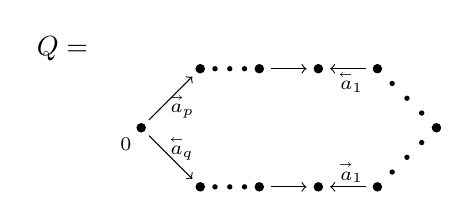
\begin{tikzpicture}
      \node at (-1,1) {$Q=$};
      \draw[fill=black] (0,0) circle (1.5pt);
      \node[below left] at (0,0) {$\scriptstyle 0$};
      \draw[->] (0.1,-0.1) -- (0.65,-0.65);
      \node[below right] at (0.25,0) {$\scriptstyle \cev{a}_q$};
      \draw[fill=black] (0.75,-0.75) circle (1.5pt);
      \draw[fill=black] (0.9375,-0.75) circle (0.75pt);
      \draw[fill=black] (1.125,-0.75) circle (0.75pt);
      \draw[fill=black] (1.3125,-0.75) circle (0.75pt);
      \draw[fill=black] (1.5,-0.75) circle (1.5pt);
      \draw[->] (1.65,-0.75) -- (2.1,-0.75);
      \draw[fill=black] (2.25,-0.75) circle (1.5pt);
      \draw[<-] (2.4,-0.75) -- (2.85,-0.75);
      \node at (2.675,-0.575) {$\scriptstyle \vec{a}_1$};
      \draw[fill=black] (3,-0.75) circle (1.5pt);
      \draw[fill=black] (3.1875,-0.5625) circle (0.75pt);
      \draw[fill=black] (3.375,-0.375) circle (0.75pt);
      \draw[fill=black] (3.5625,-0.1875) circle (0.75pt);
      \draw[fill=black] (3.75,0) circle (1.5pt);
      \draw[fill=black] (3.5625,0.1875) circle (0.75pt);
      \draw[fill=black] (3.375,0.375) circle (0.75pt);
      \draw[fill=black] (3.1875,0.5625) circle (0.75pt);
      \draw[fill=black] (3,0.75) circle (1.5pt);
      \draw[<-] (2.4,0.75) -- (2.85,0.75);
      \node at (2.675,0.575) {$\scriptstyle \cev{a}_1$};
      \draw[fill=black] (2.25,0.75) circle (1.5pt);
      \draw[->] (1.65,0.75) -- (2.1,0.75);
      \draw[fill=black] (1.5,0.75) circle (1.5pt);
      \draw[fill=black] (1.3125,0.75) circle (0.75pt);
      \draw[fill=black] (1.125,0.75) circle (0.75pt);
      \draw[fill=black] (0.9375,0.75) circle (0.75pt);
      \draw[fill=black] (0.75,0.75) circle (1.5pt);
      \draw[->] (0.1,0.1) -- (0.65,0.65);
      \node[above right] at (0.25,0) {$\scriptstyle \vec{a}_p$};
    \end{tikzpicture}\\}%end erase
    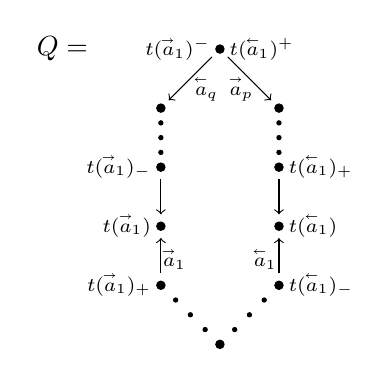
\begin{tikzpicture}
      \node at (-2,0) {$Q=$};
      \draw[fill=black] (0,0) circle (1.5pt);
      \node[right] at (0,0) {$\scriptstyle t(\cev{a}_1)^+$};
      \node[left] at (0,0) {$\scriptstyle t(\vec{a}_1)^-$};
      \draw[->] (-0.1,-0.1) -- (-0.65,-0.65);
      \node[below left] at (0.1,-0.25) {$\scriptstyle \cev{a}_q$};
      \draw[fill=black] (-0.75,-0.75) circle (1.5pt);
      \draw[fill=black] (-0.75,-0.9375) circle (0.75pt);
      \draw[fill=black] (-0.75,-1.125) circle (0.75pt);
      \draw[fill=black] (-0.75,-1.3125) circle (0.75pt);
      \draw[fill=black] (-0.75,-1.5) circle (1.5pt);
      \node[left] at (-0.75,-1.5) {$\scriptstyle t(\vec{a}_1)_-$};
      \draw[->] (-0.75,-1.65) -- (-0.75,-2.1);
      \draw[fill=black] (-0.75,-2.25) circle (1.5pt);
      \node[left] at (-0.75,-2.25) {$\scriptstyle t(\vec{a}_1)$};
      \draw[<-] (-0.75,-2.4) -- (-0.75,-2.85);
      \node at (-0.575,-2.675) {$\scriptstyle \vec{a}_1$};
      \draw[fill=black] (-0.75,-3) circle (1.5pt);
      \node[left] at (-0.75,-3) {$\scriptstyle t(\vec{a}_1)_+$};
      \draw[fill=black] (-0.5625,-3.1875) circle (0.75pt);
      \draw[fill=black] (-0.375,-3.375) circle (0.75pt);
      \draw[fill=black] (-0.1875,-3.5625) circle (0.75pt);
      \draw[fill=black] (0,-3.75) circle (1.5pt);
      \draw[fill=black] (0.1875,-3.5625) circle (0.75pt);
      \draw[fill=black] (0.375,-3.375) circle (0.75pt);
      \draw[fill=black] (0.5625,-3.1875) circle (0.75pt);
      \draw[fill=black] (0.75,-3) circle (1.5pt);
      \node[right] at (0.75,-3) {$\scriptstyle t(\cev{a}_1)_-$};
      \draw[<-] (0.75,-2.4) -- (0.75,-2.85);
      \node at (0.575,-2.675) {$\scriptstyle \cev{a}_1$};
      \draw[fill=black] (0.75,-2.25) circle (1.5pt);
      \node[right] at (0.75,-2.25) {$\scriptstyle t(\cev{a}_1)$};
      \draw[->] (0.75,-1.65) -- (0.75,-2.1);
      \draw[fill=black] (0.75,-1.5) circle (1.5pt);
      \node[right] at (0.75,-1.5) {$\scriptstyle t(\cev{a}_1)_+$};
      \draw[fill=black] (0.75,-1.3125) circle (0.75pt);
      \draw[fill=black] (0.75,-1.125) circle (0.75pt);
      \draw[fill=black] (0.75,-0.9375) circle (0.75pt);
      \draw[fill=black] (0.75,-0.75) circle (1.5pt);
      \draw[->] (0.1,-0.1) -- (0.65,-0.65);
      \node[below right] at (0,-0.25) {$\scriptstyle \vec{a}_p$};
    \end{tikzpicture}
  \end{center}
  
  For a vertex $i$ in $Q$, write $i_+$ for the next vertex of $Q$ counterclockwise from $i$ and write $i^+$ for the next source or sink of $Q$ counterclockwise from $i$.  Define $i_-$ and $i^-$ similarly by looking clockwise from $i$.  Note that $t(\vec{a}_\ell)_+=s(\vec{a}_\ell)$ and $t(\cev{a}_\ell)_-=s(\cev{a}_\ell)$.  Also note that when $i$ is a source (resp. a sink) in $Q$, both $i^-$ and $i^+$ will be sinks (resp. sources) in $Q$.  

  For vertices $i$ and $j$ in $Q$, write $[i,j]\subset Q_0$ for the subset of vertices contained weakly between $i$ and $j$ when tracing counterclockwise around $Q$ from $i$ to $j$.  Define $(i,j)$, $(i,j]$, and $[i,j)$ similarly.  Let $M_{[i,j]}$ denote the indecomposable representation of $Q$ which contains a one-dimensional vector space at each vertex $k\in[i,j]$ and a nonzero map at each arrow traversed from $i$ to $j$.  In particular, $\{i,j\}\subset\supp\soc\big(M_{[i,j]}\big)\cup\supp\top\big(M_{[i,j]}\big)$ and we take $M_{[i,i]}$ to be the simple representation $S_i$ at vertex $i$.  When enumerating over the elements of $[i,j]$ we will usually write $\sum\limits_{k=i}^j$ instead of the more proper $\sum\limits_{k\in[i,j]}$.

  For $\ell\in\ZZ$ define indecomposable representations $\vec{M}_{1,\ell}:=M_{[s(\vec{a}_{\ell-1}),t(\vec{a}_\ell)]}$ and $\cev{M}_{1,\ell}:=M_{[t(\cev{a}_\ell),s(\cev{a}_{\ell-1})]}$.  Note that when $t(\vec{a}_\ell)$ (resp. $t(\cev{a}_\ell)$) is not a sink in $Q$ the representation $\vec{M}_{1,\ell}$ (resp. $\cev{M}_{1,\ell}$) will be simple and otherwise $\vec{M}_{1,\ell}$ (resp. $\cev{M}_{1,\ell}$) will be a string module with socle $S_{t(\vec{a}_\ell)}$ (resp. $S_{t(\cev{a}_\ell)}$) and top $S_{s(\vec{a}_{\ell-1})}$ (resp. $S_{s(\cev{a}_{\ell-1})}$).  From this we see that the collections $\{\vec{M}_{1,\ell}:1\le\ell\le p\}$ and $\{\cev{M}_{1,\ell}:1\le\ell\le q\}$ give families of pairwise orthogonal bricks, i.e. there are no nonzero morphisms between non-isomorphic representations and each of these representations has trivial endomorphism ring.

  Denote by $\overrightarrow{\rep}Q$ (resp. $\overleftarrow{\rep}Q$) the full, extension-closed, additive subcategory of $\rep Q$ called the \emph{clockwise} (resp. \emph{counterclockwise}) \emph{tubular subcategory} (tube) generated by $\{\vec{M}_{1,\ell}:1\le\ell\le p\}$ (resp. $\{\cev{M}_{1,\ell}:1\le\ell\le q\}$).  Following \cite[Section 3.1]{Rin84} the clockwise and counterclockwise tubes are serial, abelian categories with simple objects given by $\{\vec{M}_{1,\ell}:1\le\ell\le p\}$ and $\{\cev{M}_{1,\ell}:1\le\ell\le q\}$ respectively.  In each case these ``simple'' objects form the mouth of the corresponding tubular categories.

  For $\ell\in\ZZ$, label the dimension vector of the ``simple'' object $\vec{M}_{1,\ell}$ as
  \begin{equation}
    \vec{\beta}_{1,\ell}=\sum_{i=s(\vec{a}_{\ell-1})}^{t(\vec{a}_\ell)}\alpha_i
  \end{equation}
  and the dimension vector of the ``simple'' object $\cev{M}_{1,\ell}$ as
  \begin{equation}
    \cev{\beta}_{1,\ell}=\sum_{i=t(\cev{a}_\ell)}^{s(\cev{a}_{\ell-1})}\alpha_i.
  \end{equation}
  The coindices of these representations can be described as follows:
  \begin{align}
    \vec{\lambda}_{1,\ell}&=\omega_{t(\vec{a}_\ell)}-\omega_{s(\vec{a}_\ell)}\\
    \cev{\lambda}_{1,\ell}&=\omega_{t(\cev{a}_\ell)}-\omega_{s(\cev{a}_\ell)}.
  \end{align}

  Define indecomposable representations $\vec{M}_{k,\ell}$ and $\cev{M}_{k,\ell}$ for $k\ge0$ and $\ell\in\ZZ$ inductively via the short exact sequences
  \[0\longrightarrow\vec{M}_{k-1,\ell}\longrightarrow\vec{M}_{k,\ell}\longrightarrow\vec{M}_{1,k+\ell-1}\longrightarrow0\]
  and
  \[0\longrightarrow\cev{M}_{k-1,\ell}\longrightarrow\cev{M}_{k,\ell}\longrightarrow\cev{M}_{1,k+\ell-1}\longrightarrow0.\]
  It follows that the dimension vectors of these representations are given for $1\le k\le p-1$ by
  \begin{align}
    \vec\beta_{k,\ell}=\sum_{m=1}^k\vec\beta_{1,\ell+m-1}=\sum_{i=s(\vec{a}_{\ell-1})}^{t(\vec{a}_{k+\ell-1})}\alpha_i
  \end{align}
  and for $1\le k\le q-1$ by
  \begin{align}
    \cev\beta_{k,\ell}=\sum\limits_{m=1}^k\cev\beta_{1,\ell+m-1}=\sum_{i=t(\cev{a}_{k+\ell-1})}^{s(\cev{a}_{\ell-1})}\alpha_i.
  \end{align}
  Similarly the coindices of these representations can be computed for $1\le k\le p-1$ as
  \begin{align}
    \vec\lambda_{k,\ell}
    &=\sum\limits_{m=1}^k\vec\lambda_{1,\ell+m-1}\\
    &=\sum\limits_{m=1}^k\omega_{t(\vec{a}_{\ell+m-1})}-\omega_{s(\vec{a}_{\ell+m-1})}
  \end{align}
  and for $1\le k\le q-1$ as
  \begin{align}
    \cev\lambda_{k,\ell}
    &=\sum\limits_{m=1}^k\cev\lambda_{1,\ell+m-1}\quad\text{}\\
    &=\sum\limits_{m=1}^k\omega_{t(\cev{a}_{\ell+m-1})}-\omega_{s(\cev{a}_{\ell+m-1})}.
  \end{align}

  \begin{proposition}\mbox{}
    \begin{enumerate}
      \item The modules listed above provide a complete set of simple objects in the categories $\overrightarrow{\rep}Q$ and $\overleftarrow{\rep}Q$.  Moreover, every object of $\overrightarrow{\rep}Q$ and $\overleftarrow{\rep}Q$ admits a unique Jordan-H\"older series with the corresponding simples as composition factors.
      \item Every regular representation of $Q$ is contained in one of $\overrightarrow{\rep}Q$ or $\overleftarrow{\rep}Q$.
      \item The exceptional regular representations of $Q$ are exactly the representations from $\overrightarrow{\rep}Q$ and $\overleftarrow{\rep}Q$ of length at most $q-1$ and $p-1$ respectively, where length refers to the Jordan-H\"older length in the respective categories.  
    \end{enumerate}
  \end{proposition}
  \begin{proof}
    \begin{enumerate}
      \item Cite Ringel's ``Tame Algebras and Integral Quadratic Forms''?  \cite[Theorem 3.6.5]{Rin84} where the described generators form the base of the tubes.
    \end{enumerate}
  \end{proof}
  \begin{remark}\label{rem:rigid regulars}
    Note that none of the rigid regular representations is sincere and all of them take the form $M_{[i,j]}$ for some $i$ and $j$ with $i\ne j_+$.
  \end{remark}

  \begin{corollary}
    A representation $M$ of $Q$ is regular if and only if $\sum\limits_{\ell=1}^r\dim M_{i_\ell}$ is even.
  \end{corollary}

  The next goal is to enumerate the subrepresentations of each rigid $M_{[i,j]}$.  To that end, following \Cref{rem:rigid regulars}, we consider $i,j\in Q_0$ with $i\ne j_+$.  Now write $Q_{[i,j]}$ for the full subquiver of $Q$ with vertices $[i,j]$ and note that this is a quiver of type $A$.  Let $i=j_1,j_2,\ldots,j_s=j$ denote the sinks and sources in $Q_{[i,j]}$.  Then the subrepresentations $N$ of $M_{[i,j]}$ are enumerated by the following data.  Choose a subset $I$ of the sinks of $Q_{[i,j]}$ to enumerate the socle of $N$.  Denote by $\bar{I}$ the subset of the sources of $Q_{[i,j]}$ consisting of all $j_t$ such that $j_{t-1},j_{t+1}\in I$.  We also take $j_1\in\bar{I}$ (resp. $j_s\in\bar{I}$) if $j_1$ (resp. $j_s$) is a source in $Q_{[i,j]}$ and $j_2\in I$ (resp. $j_{s-1}\in I$).  Choose a subset $O\subset\bar{I}$.  Write $I_L(O)=\{j_t\in I:j_{t-1}\notin O\}$ and $I_R(O)=\{j_t\in I:j_{t+1}\notin O\}$.  For each $j_t\in I_L(O)$ choose $k_{t-1}:j_{t-1}<k_{t-1}\le j_t$ and for each $j_t\in I_R(O)$ choose $k_t:j_t\le k_t<j_{t+1}$, when the inequalities are strict or both are equalities these $k_t$ enumerate, together with $O$, the top of $N$.

  The minimal injective copresentation of $M_{[i,j]}$ can be understood in terms of the quiver $Q_{[i,j]}$ as well.  This requires a couple of cases:
  \begin{itemize}
    \item $i$ and $j$ are sinks in $Q_{[i,j]}$ then a minimal injective copresentation of $M_{[i,j]}$ is given by
    \[0\longrightarrow M_{[i,j]}\longrightarrow\bigoplus_{t=1}^{\frac{s+1}{2}} I_{j_{2t-1}}\longrightarrow\bigoplus_{t=1}^{\frac{s-1}{2}} I_{j_{2t}}\longrightarrow0\]
    \item $i$ is a sink in $Q_{[i,j]}$ and $j$ is a source in $Q_{[i,j]}$ but not a source in $Q$ then a minimal injective copresentation of $M_{[i,j]}$ is given by
    \[0\longrightarrow M_{[i,j]}\longrightarrow\bigoplus_{t=1}^{\frac{s}{2}} I_{j_{2t-1}}\longrightarrow I_{j+1}\oplus\bigoplus_{t=1}^{\frac{s-2}{2}} I_{j_{2t}}\longrightarrow0\]
    \item $i$ is a sink in $Q_{[i,j]}$ and $j$ is a source in $Q$ then a minimal injective copresentation of $M_{[i,j]}$ is given by
    \[0\longrightarrow M_{[i,j]}\longrightarrow\bigoplus_{t=1}^{\frac{s}{2}} I_{j_{2t-1}}\longrightarrow \bigoplus_{t=1}^{\frac{s-2}{2}} I_{j_{2t}}\longrightarrow0\]
    \item $i$ is a source in $Q_{[i,j]}$ but not a source in $Q$ and $j$ is a sink in $Q_{[i,j]}$ then a minimal injective copresentation of $M_{[i,j]}$ is given by
    \[0\longrightarrow M_{[i,j]}\longrightarrow\bigoplus_{t=1}^{\frac{s}{2}} I_{j_{2t}}\longrightarrow I_{i-1}\oplus\bigoplus_{t=1}^{\frac{s-2}{2}} I_{j_{2t+1}}\longrightarrow0\]
    \item $i$ is a source in $Q$ and $j$ is a sink in $Q$ then a minimal injective copresentation of $M_{[i,j]}$ is given by
    \[0\longrightarrow M_{[i,j]}\longrightarrow\bigoplus_{t=1}^{\frac{s}{2}} I_{j_{2t}}\longrightarrow\oplus\bigoplus_{t=1}^{\frac{s-2}{2}} I_{j_{2t+1}}\longrightarrow0\]
    \item $i$ is a source in $Q_{[i,j]}$ but not a source in $Q$ and $j$ is a source in $Q_{[i,j]}$ but not a source in $Q$ then a minimal injective copresentation of $M_{[i,j]}$ is given by
    \[0\longrightarrow M_{[i,j]}\longrightarrow\bigoplus_{t=1}^{\frac{s-1}{2}} I_{j_{2t}}\longrightarrow I_{i-1}\oplus I_{j+1}\oplus\bigoplus_{t=1}^{\frac{s-3}{2}} I_{j_{2t+1}}\longrightarrow0\]
    \item $i$ is a source in $Q$ and $j$ is a source in $Q_{[i,j]}$ but not a source in $Q$ then a minimal injective copresentation of $M_{[i,j]}$ is given by
    \[0\longrightarrow M_{[i,j]}\longrightarrow\bigoplus_{t=1}^{\frac{s-1}{2}} I_{j_{2t}}\longrightarrow I_{j+1}\oplus\bigoplus_{t=1}^{\frac{s-3}{2}} I_{j_{2t+1}}\longrightarrow0\]
    \item $i$ is a source in $Q_{[i,j]}$ but not a source in $Q$ and $j$ is a source in $Q$ then a minimal injective copresentation of $M_{[i,j]}$ is given by
    \[0\longrightarrow M_{[i,j]}\longrightarrow\bigoplus_{t=1}^{\frac{s-1}{2}} I_{j_{2t}}\longrightarrow I_{i-1}\oplus\bigoplus_{t=1}^{\frac{s-3}{2}} I_{j_{2t+1}}\longrightarrow0\]
    \item $i$ and $j$ are sources in $Q$ then a minimal injective copresentation of $M_{[i,j]}$ is given by
    \[0\longrightarrow M_{[i,j]}\longrightarrow\bigoplus_{t=1}^{\frac{s-1}{2}} I_{j_{2t}}\longrightarrow\bigoplus_{t=1}^{\frac{s-3}{2}} I_{j_{2t+1}}\longrightarrow0\]
  \end{itemize}

  Call a vertex $i$ of a connected subquiver $Q'$ of $Q$ an \emph{internal source of $Q'$} if $i$ is a source of $Q$ and $Q'$ contains a sink both clockwise and counterclockwise from $i$.
  \begin{lemma}\mbox{}
    \begin{enumerate}
      \item For $1\le k\le p-1$ we have
      \[\vec{\lambda}_{k,\ell}=\sum_{i\in I}\omega_i-\sum_{i\in O}\omega_i\]
      where $I$ denotes the sinks in the support quiver $Q_{k,\ell}$ of $\vec{M}_{k,\ell}$ and $O$ denotes the set of internal sources of $\vec{Q}_{k,\ell}$ together with $s(\vec{a}_{k+\ell-1})$.
      \item For $1\le k\le q-1$ we have
      \[\cev{\lambda}_{k,\ell}=\sum_{i\in I}\omega_i-\sum_{i\in O}\omega_i\]
      where $I$ denotes the sinks in the support quiver $Q_{k,\ell}$ of $\cev{M}_{k,\ell}$ and $O$ denotes the set of internal sources of $\cev{Q}_{k,\ell}$ together with $s(\cev{a}_{k+\ell-1})$.
    \end{enumerate}
  \end{lemma}

  Let $\sigma\in\Sigma_{n+1}$ denote a permutation of the vertices of $Q$ such that $\sigma_0$ is a sink in $Q$ and $\sigma_i$ is a sink in $\mu_{\sigma_{i-1}}\cdots\mu_{\sigma_0} Q$ for $1\le i\le n$.  Let $c=s_{\sigma_0}\cdots s_{\sigma_n}$ denote the Coxeter element adapted to $Q$.
  \erase{%begin erase
  \begin{theorem}
    Let $g=x_{\overline{\sigma_0\!}\,}(u_{\sigma_0})\cdots x_{\overline{\sigma_n\!}\,}(u_{\sigma_n}) x_{\sigma_n}(t_{\sigma_n}) \cdots x_{\sigma_0}(t_{\sigma_0})$ denote a generic element of $L^{c,c^{-1}}$.
    \begin{enumerate}
      \item For $1\le k\le p-1$ and $1\le\ell\le p$ we have
      \begin{align}
        &\Delta_{\vec{\lambda}_{k,\ell}}(g)=\sum_{P\subset O}\left(\prod_{i\in P} t_i\prod_{i\in O\setminus P} u_i\left(\prod_{i:t(\vec{a}_\ell)<i<t(\vec{a}_\ell)^+}t_i+\sum_{m:t(\vec{a}_\ell)<m<t(\vec{a}_\ell)^+}u_m\prod_{i=m+1}^{t(\vec{a}_\ell)^+-1} t_i\right)^\delta\times\right.\\
        \nonumber&\times\left.\sum_{J\subset\bar{P}}\prod_{\substack{i:j^-<i<j^+\\j\in J}}t_i\prod_{i\in I\setminus J}u_i^{-1}\left(\prod_{j\in O^-(J)}\sum_{m:j^-<m\le j}u_{m-1}\prod_{i=m}^{j-1} t_i\right)\left(\prod_{j\in O^+(J)}\sum_{m:j\le m<j^+}u_{m+1}\prod_{i=j+1}^{m} t_i\right)\right)
      \end{align}
      where:
      \begin{itemize}
        \item $O$ denotes the set of internal sources in the support quiver $\vec{Q}_{k,\ell}$ of $\vec{M}_{k,\ell}$ together with $s(\vec{a}_{k+\ell-1})$ read counterclockwise around $Q$;
        \item for $P\subset O$, $\bar{P}$ denotes the set of sinks $j$ in $\vec{Q}_{k,\ell}$ for which $j^-,j^+\in P$;
        \item $I$ denotes the sinks in $\vec{Q}_{k,\ell}$ read counterclockwise around $Q$;
        \item for $J\subset\bar{P}$, $O^\pm(J)=\{j\in O:j^\pm\in I\setminus J\}$;
        \item $\delta=\begin{cases}1 & \text{if $t(\vec{a}_\ell)$ is a not a sink in $Q$ and $t(\vec{a}_\ell)^+\in P$;}\\0 & \text{otherwise.}\end{cases}$
      \end{itemize}
      \item For $1\le k\le q-1$ and $1\le\ell\le q$  we have
      \begin{align}
        &\Delta_{\cev{\lambda}_{k,\ell}}(g)=\sum_{P\subset O}\left(\prod_{i\in P} t_i\prod_{i\in O\setminus P} u_i\left(\prod_{i:t(\vec{a}_\ell)^-<i<t(\vec{a}_\ell)}t_i+\sum_{m:t(\vec{a}_\ell)^-<m<t(\vec{a}_\ell)}u_m\prod_{i=t(\vec{a}_\ell)^-+1}^{m-1} t_i\right)^\delta\times\right.\\
        \nonumber&\times\left.\sum_{J\subset\bar{P}}\prod_{\substack{i:j^-<i<j^+\\j\in J}}t_i\prod_{i\in I\setminus J}u_i^{-1}\left(\prod_{j\in O^-(J)}\sum_{m:j^-<m\le j}u_{m-1}\prod_{i=m}^{j-1} t_i\right)\left(\prod_{j\in O^+(J)}\sum_{m:j\le m<j^+}u_{m+1}\prod_{i=j+1}^{m} t_i\right)\right)
      \end{align}
      where:
      \begin{itemize}
        \item $O$ denotes the set of internal sources in the support quiver $\cev{Q}_{k,\ell}$ of $\cev{M}_{k,\ell}$ together with $s(\cev{a}_{k+\ell-1})$ read counterclockwise around $Q$;
        \item for $P\subset O$, $\bar{P}$ denotes the set of sinks $j$ in $\cev{Q}_{k,\ell}$ for which $j^-,j^+\in P$;
        \item $I$ denotes the sinks in $\cev{Q}_{k,\ell}$ read counterclockwise around $Q$;
        \item for $J\subset\bar{P}$, $O^\pm(J)=\{j\in O:j^\pm\in I\setminus J\}$;
        \item $\delta=\begin{cases}1 & \text{if $t(\cev{a}_\ell)$ is a not a sink in $Q$ and $t(\cev{a}_\ell)^-\in P$;}\\0 & \text{otherwise.}\end{cases}$
      \end{itemize}
    \end{enumerate}
  \end{theorem}
  \begin{proof}
    The calculation breaks into several independent type $A$ weight space computations coming from consecutive strings of clockwise or consecutive counterclockwise arrows in $Q$.  The set $I$ records the positive components of the weight $\vec{\lambda}_{k,\ell}$ which all correspond to sinks in $Q_{k,\ell}$ while the set $O$ records the negative components of the weight $\vec{\lambda}_{k,\ell}$ which all correspond to sources in $Q_{k,\ell}$.  In each case, such a string of equi-oriented arrows is only considered if a step up in weight was performed at the source $i\in I$ of that path, i.e. if the action of $x_i(t_i)$ replaced the current weight $\omega$ by $\omega+\alpha_i=\omega-2\omega_i+\omega_{i-1}+\omega_{i+1}$ in which case the $x_{\bar{i}}(u_i)$ will contribute nothing later.  This accounts for the sum over all subsets $P\subset O$ as well as the first product of $t_i$'s and the first product of the $u_i$'s (steps not taken when acting by $x_i(t_i)$ and thus no change in weight by $x_{\bar{i}}(u_i)$).

    Next, one has to consider each of these strings separately (mostly).  If no change in weight is made by the action of $x_{\bar{i}}(u_i)$ for $i\in I$ there will be a factor of $u_i^{-1}$.  The set $J\subset\bar{P}$ records those sinks $j$ where every $x_i(t_i)$ along \emph{both} equi-oriented paths ending at $j$ replaced the current weight $\omega$ by $\omega-\alpha_i$ in which case each of the $x_{\bar{i}}(u_i)$ along these paths will contribute nothing later.  This accounts for the products over elements of $J$ and $I\setminus J$.

    Finally, along each equi-oriented path one can choose to act by some of the $x_i(t_i)$ in a contiguous string beginning at the source, this accounts for the two products of sums, one for clockwise paths and one for counterclockwise paths.  The $\delta$ is a slight annoyance present in the weight $\vec{\lambda}_{k,\ell}$, there is one equi-oriented string whose sink $t(\vec{a}_{k,\ell})$ appears in $\vec{\lambda}_{k,\ell}$ with positive coefficient but which is not an internal sink so it was hard to find uniform notation to capture that string with the others.
  \end{proof}}%end erase
  {%begin erase
  \begin{theorem}
    Let $g=x_{\overline{\sigma_0\!}\,}(u_{\sigma_0})\cdots x_{\overline{\sigma_n\!}\,}(u_{\sigma_n}) x_{\sigma_n}(t_{\sigma_n}) \cdots x_{\sigma_0}(t_{\sigma_0})$ denote a generic element of $L^{c,c^{-1}}$.
    \begin{enumerate}
      \item For $1\le k\le p-1$ we have
      \begin{align}
        &\Delta_{-\vec{\lambda}_{k,\ell}}(g)=\sum_{J\subset I}\left(\prod_{i\in J} t_i\prod_{i\in I\setminus J} u_i\left(u_{t(\vec{a}_\ell)_-}+\sum_{m=\left(t(\vec{a}_\ell)^-\right)_+}^{t(\vec{a}_\ell)_-}u_{m_-}\prod_{i=m}^{t(\vec{a}_\ell)_-} t_i+\prod_{i=t(\vec{a}_\ell)^-}^{t(\vec{a}_\ell)_-}t_i\right)^\delta\times\right.\\
        \nonumber&\times\left.\sum_{P\subset\bar{J}}\prod_{\substack{j\in P\\i\in(j^-,j^+)}}t_i\prod_{i\in O\setminus P}u_i^{-1}\left(\prod_{j\in I^-(P)}\left(u_{j_-}+\sum_{m\in(j^-,j)}u_{m_-}\prod_{i=m}^{j_-} t_i\right)\right)\left(\prod_{j\in I^+(P)}\left(u_{j_+}+\sum_{m\in(j,j^+)}u_{m_+}\prod_{i=j_+}^m t_i\right)\right)\right)
      \end{align}
      where:
      \begin{itemize}
        \item $I$ denotes the sinks in the support quiver $\vec{Q}_{k,\ell}$ of $\vec{M}_{k,\ell}$ read counterclockwise around $Q$,
        \item $O$ denotes the set of internal sources of $\vec{Q}_{k,\ell}$ together with $s(\vec{a}_{k+\ell-1})$,
        \item for $J\subset I$, $\bar{J}$ denotes the set of sources $j$ in the support quiver $\vec{Q}_{k,\ell}$ for which $j^-,j^+\in J$,
        \item for $P\subset\bar{J}$, $I^\pm(P)=\{j\in J:j^\pm\in O\setminus P\}$,
        \item $\delta=\begin{cases}1 & \text{if $t(\vec{a}_\ell)$ is a sink in $Q$ and $t(\vec{a}_\ell)\in J$;}\\0 & \text{otherwise.}\end{cases}$
      \end{itemize}
      \item For $1\le k\le q-1$ we have
      \begin{align}
        &\Delta_{-\cev{\lambda}_{k,\ell}}(g)=\sum_{J\subset I}\left(\prod_{i\in J} t_i\prod_{i\in I\setminus J} u_i\left(u_{t(\cev{a}_\ell)_+}+\sum_{m=t(\cev{a}_\ell)_+}^{\left(t(\cev{a}_\ell)^+\right)_-}u_{m_+}\prod_{i=t(\cev{a}_\ell)_+}^m t_i+\prod_{i=t(\cev{a}_\ell)_+}^{t(\cev{a}_\ell)^+}t_i\right)^\delta\times\right.\\
        \nonumber&\times\left.\sum_{P\subset\bar{J}}\prod_{\substack{j\in P\\i\in(j^-,j^+)}}t_i\prod_{i\in O\setminus P}u_i^{-1}\left(\prod_{j\in I^-(P)}\left(u_{j_-}+\sum_{m\in(j^-,j)}u_{m_-}\prod_{i=m}^{j_-}t_i\right)\right)\left(\prod_{j\in I^+(P)}\left(u_{j^+}+\sum_{m\in(j,j^+)}u_{m_+}\prod_{i=j_+}^m t_i\right)\right)\right)
      \end{align}
      where:
      \begin{itemize}
        \item $I$ denotes the sinks in the support quiver $\cev{Q}_{k,\ell}$ of $\cev{M}_{k,\ell}$ read clockwise around $Q$,
        \item $O$ denotes the set of internal sources of $\cev{Q}_{k,\ell}$ together with $s(\cev{a}_{k+\ell-1})$,
        \item for $J\subset I$, $\bar{J}$ denotes the set of sources $j$ in the support quiver $\cev{Q}_{k,\ell}$ for which $j^-,j^+\in J$,
        \item for $P\subset\bar{J}$, $I^\pm(P)=\{j\in J:j^\pm\in O\setminus P\}$,
        \item $\delta=\begin{cases}1 & \text{if $t(\cev{a}_\ell)$ is a sink in $Q$ and $t(\cev{a}_\ell)\in J$;}\\0 & \text{otherwise.}\end{cases}$
      \end{itemize}
    \end{enumerate}
  \end{theorem}
  \begin{proof}
    The calculation breaks into several independent type $A$ weight space computations coming from consecutive strings of clockwise or consecutive counterclockwise arrows in $Q$.  The set $I$ records the negative components of the weight $-\vec{\lambda}_{k,\ell}$ which all correspond to sinks in $Q_{k,\ell}$ while the set $O$ records the positive components of the weight $\vec{\lambda}_{k,\ell}$ which all correspond to sources in $Q_{k,\ell}$.  In each case, such a string of equi-oriented arrows is only considered if a step up in weight was performed at the sink $i\in I$ of that path, i.e. if the action of $x_i(t_i)$ replaced the current weight $\omega$ by $\omega+\alpha_i=\omega-2\omega_i+\omega_{i-1}+\omega_{i+1}$ in which case the $x_{\bar{i}}(u_i)$ will contribute nothing later.  This accounts for the sum over all subsets $J\subset I$ as well as the first product of $t_i$'s and the first product of the $u_i$'s (steps not taken when acting by $x_i(t_i)$ and thus no change in weight by $x_{\bar{i}}(u_i)$).

    Next, one has to consider each of these strings separately (mostly).  If no change in weight is made by the action of $x_{\bar{i}}(u_i)$ for $i\in O$ there will be a factor of $u_i^{-1}$.  The set $P\subset\bar{J}$ records those sources $j$ where every $x_i(t_i)$ along \emph{both} equi-oriented paths beginning at $j$ replaced the current weight $\omega$ by $\omega+\alpha_i$ in which case each of the $x_{\bar{i}}(u_i)$ along these paths will contribute nothing later.  This accounts for the products over elements of $P$ and $O\setminus P$.

    Finally, along each equi-oriented path one can choose to act by some of the $x_i(t_i)$ in a contiguous string beginning at the sink, this accounts for the two products of sums, one for clockwise paths and one for counterclockwise paths.  The $\delta$ is a slight annoyance present in the weight $-\vec{\lambda}_{k,\ell}$, there is one equi-oriented string whose sink $t(\vec{a}_\ell)$ (resp. $t(\cev{a}_\ell)$) may appear in $-\vec{\lambda}_{k,\ell}$ with negative coefficient but where $s(\vec{a}_{\ell+1})$ (resp. $s(\cev{a}_{\ell-1}$) does not appear so it was hard to find uniform notation to capture that string with the others.
  \end{proof}}%end erase

  For a representation $M$ of $Q$ define the \emph{cluster character} $x_M\in\cT$ by
  \begin{equation}
    x_M=\sum_{\bfe\in\ZZ^{Q_0}_{\ge0}}\chi(Gr_\bfe(M))x^{B\bfe-{}^*M}
  \end{equation}
  where ${}^*M=\sum\limits_{i\in Q_0}\langle S_i,M\rangle\omega_i$, $Gr_\bfe(M)$ denotes the Grassmannian of subrepresentations of $M$ with dimension vector $\bfe$, and for a vector $(\bfb_1,\bfb_2)\in\big(\ZZ^{Q_0}\big)^2$ we write $x^\bfb=\prod_{i\in Q_0} x_i^{b_{1i}}y_i^{b_{2i}}$.
  \begin{theorem}\mbox{}
    \begin{enumerate}
      \item For $1\le k\le p-1$ we have
      \begin{align}
        &x_{\vec{M}_{k,\ell}}=x^{\sum_{i\in O}\omega_i-\sum_{i\in I}\omega_i}\sum_{J\subset I}\prod_{i\in J}x_{i_-}^{-1}y_ix_{i_+}^{-1}\times\\
        \nonumber&\times\left(1+\sum_{m=\left(t(\vec{a}_\ell)^-\right)_+}^{t(\vec{a}_\ell)_-}x_{m_-}^{-1}x_m^{-1}x_{t(\vec{a}_\ell)_-}x_{t(\vec{a}_\ell)}\prod_{i=m}^{t(\vec{a}_\ell)_-}y_i+x_{\left(t(\vec{a}_\ell)^-\right)_-}x_{t(\vec{a}_\ell)^-}^{-1}x_{t(\vec{a}_\ell)_-}x_{t(\vec{a}_\ell)}\prod_{i=t(\vec{a}_\ell)^-}^{t(\vec{a}_\ell)_-}y_i\right)^\delta\times\\
        \nonumber&\times\sum_{P\subset\bar{J}}\prod_{j\in P}\left(x_{j^-}x_{(j^-)_+}x_j^{-2}x_{(j^+)_-}x_{j^+}\prod_{i\in(j^-,j^+)}y_i\right)\prod_{j\in I^-(P)}\left(1+\sum_{m\in(j^-,j)}x_{m_-}^{-1}x_m^{-1}x_{j_-}x_j\prod_{i=m}^{j_-}y_i\right)\times\\
        \nonumber&\hspace{0.5in}\times\prod_{j\in I^+(P)}\left(1+\sum_{m\in(j,j^+)}x_jx_{j_+}x_m^{-1}x_{m_+}^{-1}\prod_{i=j_+}^m y_i\right)
      \end{align}
      where:
      \begin{itemize}
        \item $I$ denotes the sinks in the support quiver $\vec{Q}_{k,\ell}$ of $\vec{M}_{k,\ell}$ read counterclockwise around $Q$,
        \item $O$ denotes the set of internal sources of $\vec{Q}_{k,\ell}$ together with $s(\vec{a}_{k+\ell-1})$,
        \item for $J\subset I$, $\bar{J}$ denotes the set of sources $j$ in the support quiver $\vec{Q}_{k,\ell}$ for which $j^-,j^+\in J$,
        \item for $P\subset\bar{J}$, $I^\pm(P)=\{j\in J:j^\pm\in O\setminus P\}$,
        \item $\delta=\begin{cases}1 & \text{if $t(\vec{a}_\ell)$ is a sink in $Q$ and $t(\vec{a}_\ell)\in J$;}\\0 & \text{otherwise.}\end{cases}$
      \end{itemize}
      \item For $1\le k\le q-1$ we have
      \begin{align}
        &x_{\cev{M}_{k,\ell}}=x^{\sum_{i\in O}\omega_i-\sum_{i\in I}\omega_i}\sum_{J\subset I}\prod_{i\in J}x_{i_-}^{-1}y_ix_{i_+}^{-1}\times\\
        \nonumber&\times\left(1+\sum_{m=t(\cev{a}_\ell)_+}^{\left(t(\cev{a}_\ell)^+\right)_-}x_{t(\cev{a}_\ell)}x_{t(\cev{a}_\ell)_+}x_m^{-1}x_{m_+}^{-1}\prod_{i=t(\cev{a}_\ell)_+}^m y_i+x_{t(\cev{a}_\ell)}x_{t(\cev{a}_\ell)_+}x_{t(\cev{a}_\ell)^+}^{-1}x_{\left(t(\cev{a}_\ell)^+\right)_+}\prod_{i=t(\cev{a}_\ell)_+}^{t(\cev{a}_\ell)^+}y_i\right)^\delta\times\\
        \nonumber&\times\sum_{P\subset\bar{J}}\prod_{j\in P}\left(x_{j^-}x_{(j^-)_+}x_j^{-2}x_{(j^+)_-}x_{j^+}\prod_{i\in(j^-,j^+)}y_i\right)\prod_{j\in I^-(P)}\left(1+\sum_{m\in(j^-,j)}x_{m_-}^{-1}x_m^{-1}x_{j_-}x_j\prod_{i=m}^{j_-}y_i\right)\times\\
        \nonumber&\hspace{0.5in}\times\prod_{j\in I^+(P)}\left(1+\sum_{m\in(j,j^+)}x_jx_{j_+}x_m^{-1}x_{m_+}^{-1}\prod_{i=j_+}^m y_i\right)
      \end{align}
      where:
      \begin{itemize}
        \item $I$ denotes the sinks in the support quiver $\cev{Q}_{k,\ell}$ of $\cev{M}_{k,\ell}$ read clockwise around $Q$,
        \item $O$ denotes the set of internal sources of $\cev{Q}_{k,\ell}$ together with $s(\cev{a}_{k+\ell-1})$,
        \item for $J\subset I$, $\bar{J}$ denotes the set of sources $j$ in the support quiver $\cev{Q}_{k,\ell}$ for which $j^-,j^+\in J$,
        \item for $P\subset\bar{J}$, $I^\pm(P)=\{j\in J:j^-\in\bar{I}\setminus P\}$,
        \item $\delta=\begin{cases}1 & \text{if $t(\cev{a}_\ell)$ is a sink in $Q$ and $t(\cev{a}_\ell)\in J$;}\\0 & \text{otherwise.}\end{cases}$
      \end{itemize}
    \end{enumerate}
  \end{theorem}
  \begin{proof}
    The following are read off from the $i^{th}$ column of the exchange matrix:
    \begin{itemize}
      \item If a sink $i$ is in the support of a submodule, it contributes $x_{i_-}^{-1}y_ix_{i_+}^{-1}$.
      \item If a source $i$ is in the support of a submodule, it contributes $x_{i_-}y_ix_{i_+}$.
      \item If $i$ is a non-source and non-sink in the support with $i^+$ a sink, it contributes $x_{i_-}^{-1}y_ix_{i_+}$.
      \item If $i$ is a non-source and non-sink in the support with $i^-$ a sink, it contributes $x_{i_-}y_ix_{i_+}^{-1}$.
    \end{itemize}
    Then enumerate submodules to get the formulas above.
  \end{proof}

  \begin{lemma}\mbox{}
    Let $g$ be a generic element of $L^{c,c^{-1}}$.
    \begin{enumerate}
      \item $\Delta_{\omega_i}(g)=u_i^{-1}$
      \item $\Delta_{c\omega_i}^{\omega_i}(g)=\begin{cases}u_i^{-1}\prod\limits_{j=i^-}^{i^+}t_j & \text{if $i$ is a sink in $Q$;}\\u_i^{-1}t_i & \text{if $i$ is a source in $Q$;}\\u_i^{-1}\prod\limits_{j=i}^{i^+}t_j & \text{if $i$ is neither a source nor a sink in $Q$ but $i^+$ is a source;}\\u_i^{-1}\prod\limits_{j=i^-}^it_j & \text{if $i$ is neither a source nor a sink in $Q$ but $i^-$ is a source.}\end{cases}$
      \item For 
      \begin{equation}
        y_i=\begin{cases}\Delta_{c\omega_i}^{\omega_i} & \text{if $i$ is a sink in $Q$;}\\\Delta_{c\omega_i}^{\omega_i}\left(\Delta_{c\omega_{i_-}}^{\omega_{i_-}}\Delta_{c\omega_{i_+}}^{\omega_{i_+}}\right)^{-1} & \text{if $i$ is a source in $Q$;}\\\Delta_{c\omega_i}^{\omega_i}\left(\Delta_{c\omega_{i_+}}^{\omega_{i_+}}\right)^{-1} & \text{if $i$ is neither a source nor a sink in $Q$ but $i^+$ is a sink;}\\\Delta_{c\omega_i}^{\omega_i}\left(\Delta_{c\omega_{i_-}}^{\omega_{i_-}}\right)^{-1} & \text{if $i$ is neither a source nor a sink in $Q$ but $i^-$ is a sink.}\end{cases}
      \end{equation}
      we have
      \begin{align}
        y_i(g)&=\begin{cases}u_i^{-1}t_i & \text{if $i$ is a sink in $Q$;}\\u_{i_-}u_i^{-1}u_{i_+}t_i & \text{if $i$ is a source in $Q$;}\\u_i^{-1}u_{i_+}t_i & \text{if $i$ is neither a source nor a sink in $Q$ but $i^+$ is a sink;}\\u_{i_-}u_i^{-1}t_i & \text{if $i$ is neither a source nor a sink in $Q$ but $i^-$ is a sink.}\end{cases}
      \end{align}
    \end{enumerate}
  \end{lemma}

  \begin{theorem}
    For $x_i=\Delta_{\omega_i}$ and $y_i$ as above, we have $x_{\vec{M}_{k,\ell}}=\Delta_{-\vec{\lambda}_{k,\ell}}$ and $x_{\cev{M}_{k,\ell}}=\Delta_{-\cev{\lambda}_{k,\ell}}$ on $L^{c,c^{-1}}$.
  \end{theorem}
  \begin{proof}\mbox{}
    \begin{itemize}
      \item $x^{\sum_{i\in O}\omega_i-\sum_{i\in I}\omega_i}=\prod\limits_{i\in O}u_i^{-1}\prod\limits_{i\in I}u_i$
      \item For a sink $i\in J$ we have
      \[\left(x_{i_-}^{-1}y_ix_{i_+}^{-1}\right)(g)=u_{i_-}u_i^{-1}u_{i_+}t_i.\]
      \item For $j\in I^-(P)$ and $m\in(j^-,j)$ we have
      \[\left(x_{m_-}^{-1}x_m^{-1}x_{j_-}x_j\prod\limits_{i\in[m,j_-]}y_i\right)(g)=u_{m_-}u_{j_-}^{-1}\prod\limits_{i\in[m,j_-]}t_i.\]
      \item For $j\in I^+(P)$ and $m\in(j,j^+)$ we have
      \[\left(x_jx_{j_+}x_m^{-1}x_{m_+}^{-1}\prod\limits_{i\in[j_+,m]}y_i\right)(g)=u_{j_+}^{-1}u_{m_+}\prod\limits_{i\in[j_+,m]}t_i.\]
      \item For a source $j\in P$ we have
      \[\left(x_{j^-}x_{(j^-)_+}x_j^{-2}x_{(j^+)_-}x_{j^+}\prod\limits_{i\in(j^-,j^+)}y_i\right)(g)=u_{(j^-)_+}^{-1}u_ju_{(j^+)_-}^{-1}\prod\limits_{i\in(j^-,j^+)}t_i.\]
      \item 
      \[\left(x_{\left(t(\vec{a}_\ell)^-\right)_-}x_{t(\vec{a}_\ell)^-}^{-1}x_{t(\vec{a}_\ell)_-}x_{t(\vec{a}_\ell)}\prod_{i=t(\vec{a}_\ell)^-}^{t(\vec{a}_\ell)_-}y_i\right)(g)=u_{t(\vec{a}_\ell)_-}^{-1}\prod_{i=t(\vec{a}_\ell)^-}^{t(\vec{a}_\ell)_-}t_i\]
      \item
      \[\left(x_{t(\cev{a}_\ell)}x_{t(\cev{a}_\ell)_+}x_{t(\cev{a}_\ell)^+}^{-1}x_{\left(t(\cev{a}_\ell)^+\right)_+}\prod_{i=t(\cev{a}_\ell)_+}^{t(\cev{a}_\ell)^+}y_i\right)(g)=u_{t(\cev{a}_\ell)_+}^{-1}\prod_{i=t(\cev{a}_\ell)_+}^{t(\cev{a}_\ell)^+}t_i\]
    \end{itemize}
    Comparing formulas using the above substitutions completes the proof.
  \end{proof}


\section{Conventions}

\begin{itemize}

  \item 
    The Cartan matrix is $A=(a_{ij})$ and it's $n \times n$.

  \item 
    $I=[1,n]$ is the set of indices of the nodes of the Dynkin diagram. The labels are such that $c=s_1\dots s_n$.

  \item 
    $B_c$ is the matrix given by
    \[
      b_{ij} = \begin{cases}
        -a_{ij} & i<j\\
        a_{ij}  & i>j\\
        0       & i=j
      \end{cases}
    \]
    (negative below the diagonal)

  \item
    The Euler matrix $E_c$ is given by
    \[
      e_{ij} = \begin{cases}
        0       & i<j\\
        a_{ij}  & i>j\\
        1       & i=j
      \end{cases}
    \]
    (negative below the diagonal, 0 above)

  \item
    The initial $B$-matrix for $G^{c,c^{-1}}$ with double reduced word $\bar 1,\dots,\bar n,n\dots 1$ is
    \[
      \left[
        \begin{array}{c}
          B_c\\
          E_{c^{-1}}\\
          E_{c^{-1}}
        \end{array}
      \right]
    \]
  
  \item 
    The minor $\Delta_\omega^\delta$ is our notation for YZ's $\Delta_{\delta, \omega}$.
  
  \item 
    $[\alpha:\alpha_j]$ notation defined immediately before \Cref{lem:minorsondbc}
  
  \item 
    The transpose $g \mapsto g^T$ of YZ is defined in passing without notation in the proof of \Cref{lem:minorsondbc}.
  
  \item 
    $L_{\omega_i}$ is the $i$th fundamental representation in the proof of \Cref{lem:minorsondbc}.

  \item 
    Used the notation $h^\omega$ for $\omega$ a weight and $h \in H$ without explaining it in the proof of \Cref{lem:minorsondbc}.

  \item 
    We use $x_{-i}(t)$ rather than a barred version for negative 1-parameter subgroups in the proof of \Cref{lem:minorsondbc}.

  \item 
    The identity $\beta_j^+ + \sum_{i=1}^{j-1} a_{ij} \beta_i^+ = \alpha_j$ is used in the proof of \Cref{lem:minorsondbc} without comment.
\end{itemize}

% bibliography
\bibliographystyle{amsalpha}
\bibliography{bibliography}

\end{document}
